\chapter{Symétrie et groupes ponctuels}\label{ch:b3:point-groups}

Tournez un flocon de neige de soixante degrés et rien ne change~; tournez
une molécule de benzène du même angle, et ses six carbones et ses six
hydrogènes viennent exactement à la place les uns des autres. La symétrie
d'une molécule décide de plusieurs de ses propriétés avant tout calcul~:
peut-elle avoir un moment dipolaire~? peut-elle exister sous deux formes
images l'une de l'autre dans un miroir~? lesquelles de ses vibrations
absorbent dans l'infrarouge~? quelles orbitales peuvent se mélanger~?
Pour s'en servir, les chimistes ont emprunté aux mathématiques le
langage des groupes. Ce chapitre définit les \omterm{def:b3:point-groups:operation}{opérations de symétrie} d'une
molécule, les réunit en son \omterm{def:b3:point-groups:point-group}{groupe ponctuel}, donne une procédure pour
trouver ce groupe, démontre deux théorèmes sur la polarité et la
chiralité, et introduit les \omterm{def:b3:point-groups:irrep}{tables de caractères} sur lesquelles
s'appuie le \cref{ch:b3:group-theory-applied}.

\begin{recall}
Le volume de première année a prévu la géométrie des molécules par le
modèle VSEPR, défini le moment dipolaire d'une molécule polaire, et défini
la chiralité~: une molécule chirale n'est pas superposable à son image
dans un miroir. Le volume de deuxième année a utilisé la symétrie, en
mots, pour construire les orbitales de fragment de \ce{H2O} et de \ce{NH3}.
\end{recall}

\begin{omfigure}
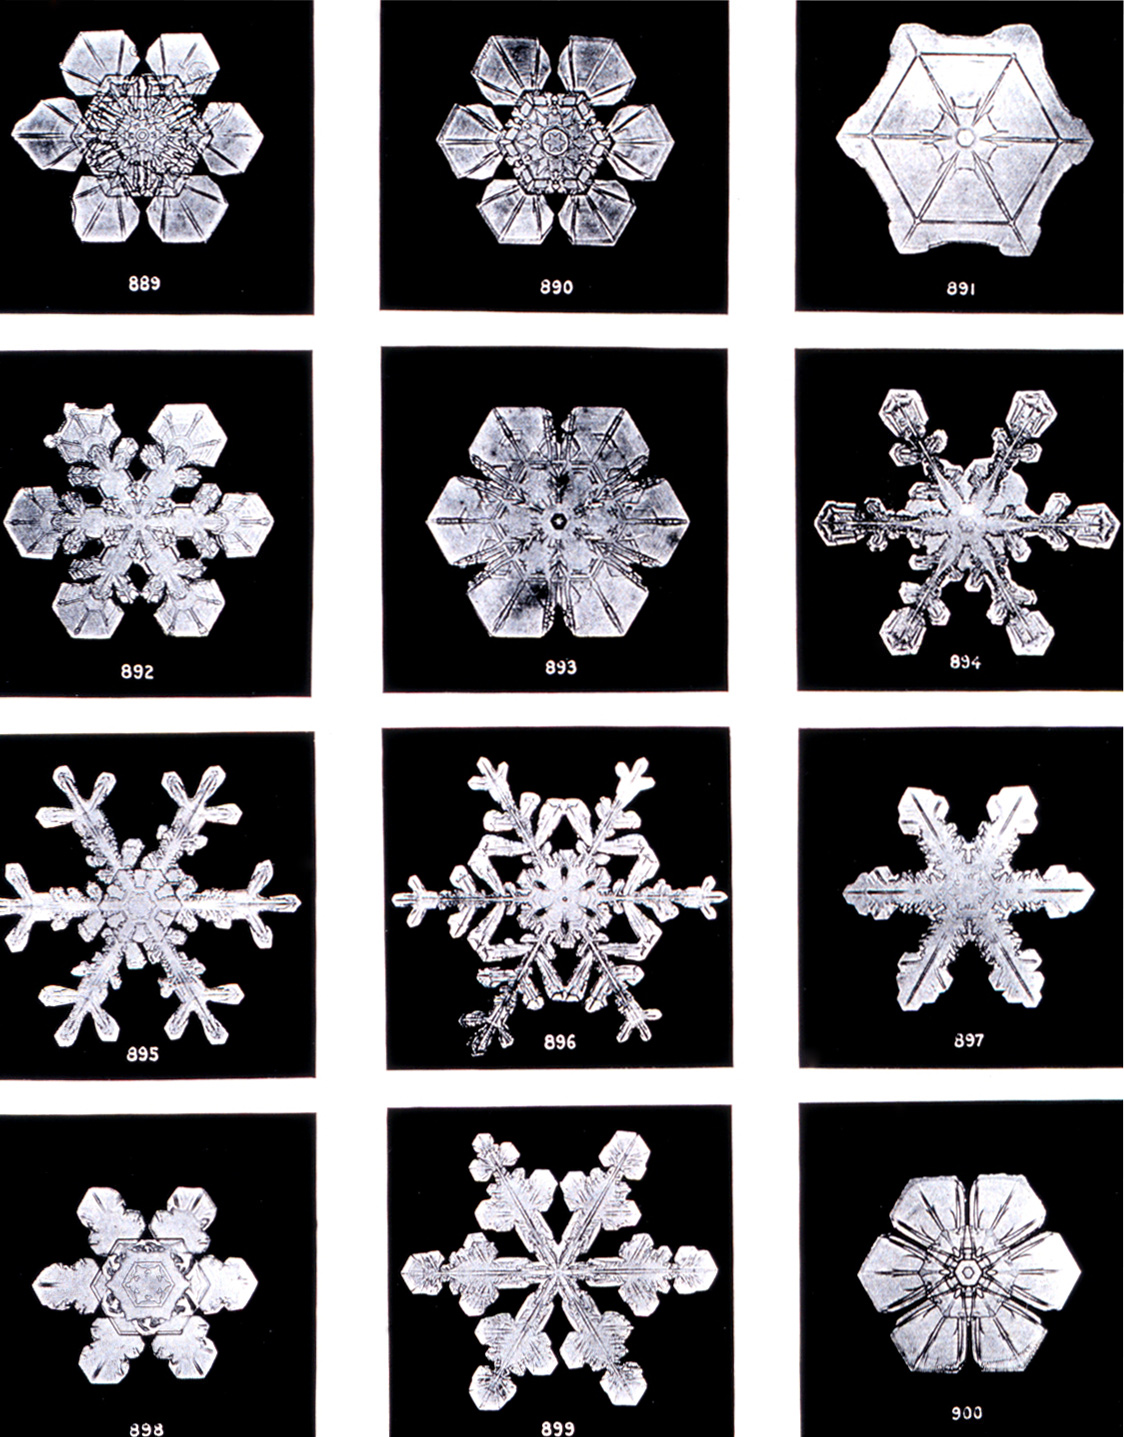
\includegraphics[width=0.4\linewidth]{images/book4/bentley-snowflakes.jpg}\hspace{1em}%
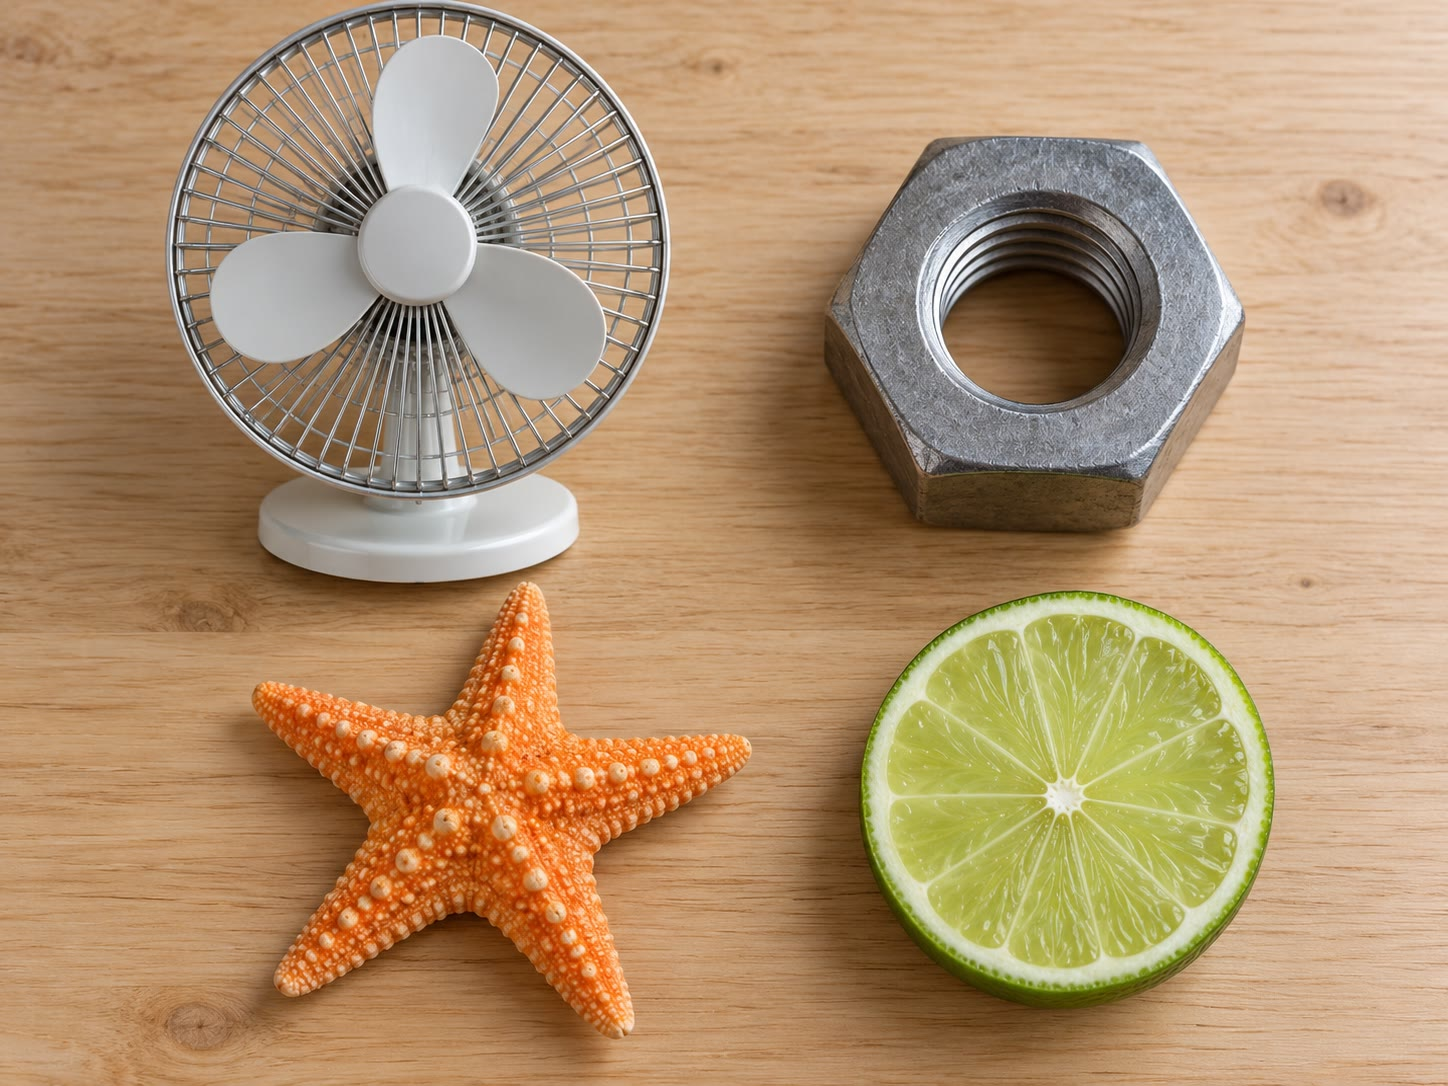
\includegraphics[width=0.48\linewidth]{images/book4/ai/b3-04-symmetric-objects.jpg}

{\small À gauche~: cristaux de neige photographiés par Wilson Bentley vers
1902, chacun de symétrie d'ordre six. À droite~: objets du quotidien
présentant une symétrie de rotation d'ordre trois, six et cinq.}
\end{omfigure}

\section{Opérations et éléments de symétrie}

\begin{definition}[Opération de symétrie, élément de symétrie]\label{def:b3:point-groups:operation}
Une \emph{opération de symétrie}\index{operation de symetrie@opération de symétrie} est un déplacement ou
une réflexion qui laisse une molécule dans une configuration impossible à
distinguer de la configuration initiale (chaque atome sur une position
occupée auparavant par un atome de même nature). Un \emph{élément de
symétrie}\index{element de symetrie@élément de symétrie} est l'objet
géométrique --- un point, une droite, un plan --- par rapport auquel
l'opération est effectuée.
\end{definition}

Toute molécule possède l'opération identité $E$, qui ne fait rien. Les
autres sont de quatre sortes.

\begin{definition}[Axe de rotation propre, axe principal]\label{def:b3:point-groups:rotation}
Un \emph{axe de rotation propre}\index{axe de rotation propre} $C_n$ est une
droite autour de laquelle une rotation de $2\pi/n$ est une \omterm{def:b3:point-groups:operation}{opération de
symétrie}, notée aussi
$C_n$~; ses puissances $C_n^k$ sont les rotations de $2\pi k/n$, et
$C_n^n = E$. L'axe de plus grand $n$ est l'\emph{axe principal}\index{axe principal},
pris comme axe $z$.
\end{definition}

\begin{definition}[Plans de symétrie]\label{def:b3:point-groups:mirror}
Un \emph{plan de symétrie}\index{plan de symetrie@plan de symétrie} $\sigma$ est un plan par rapport
auquel la réflexion est une \omterm{def:b3:point-groups:operation}{opération de symétrie}~; $\sigma^2 = E$. Un
plan de symétrie est un \emph{plan de symétrie vertical}\index{plan de symetrie vertical@plan de symétrie vertical} $\sigma_v$ s'il
contient l'\omterm{def:b3:point-groups:rotation}{axe principal}, un \emph{plan de symétrie
horizontal}\index{plan de symetrie horizontal@plan de symétrie horizontal} $\sigma_h$ s'il lui est
perpendiculaire, et un \emph{plan de symétrie dièdre}\index{plan de symetrie diedre@plan de symétrie dièdre}
$\sigma_d$ s'il contient l'\omterm{def:b3:point-groups:rotation}{axe principal} et partage en deux l'angle de
deux axes $C_2$ perpendiculaires à celui-ci.
\end{definition}

\begin{definition}[Centre d'inversion]\label{def:b3:point-groups:inversion}
Un \emph{centre d'inversion}\index{centre d'inversion} $i$ est un point
par rapport auquel l'inversion, $(x, y, z) \mapsto (-x, -y, -z)$, est une
\omterm{def:b3:point-groups:operation}{opération de symétrie}.
\end{definition}

\begin{definition}[Axe de rotation impropre]\label{def:b3:point-groups:improper}
Un \emph{axe de rotation impropre}\index{axe de rotation impropre} $S_n$
est une droite autour de laquelle une rotation de $2\pi/n$ suivie d'une
réflexion dans le plan qui lui est perpendiculaire est une \omterm{def:b3:point-groups:operation}{opération de
symétrie}. $S_1 = \sigma$ et $S_2 = i$.
\end{definition}

\begin{example}[Éléments de quatre molécules]\label{ex:b3:point-groups:elements}
\ce{H2O}~: $E$, un axe $C_2$ bissecteur de l'angle H--O--H, et deux plans
verticaux, le plan de la molécule et le plan qui lui est perpendiculaire.
\ce{NH3}~:
$E$, un axe $C_3$ passant par N (opérations $C_3$ et $C_3^2$), et trois
$\sigma_v$, contenant chacun une liaison N--H. \ce{BF3}~: un $C_3$, trois
$C_2$ selon les liaisons B--F,
$\sigma_h$ (le plan de la molécule), trois $\sigma_v$, et un $S_3$.
\ce{CH4}~: quatre
$C_3$ selon les liaisons C--H, trois $C_2$ bissecteurs d'angles H--C--H,
qui sont aussi des axes $S_4$, et six $\sigma_d$, contenant chacun deux
liaisons C--H (figure ci-dessous).
\end{example}

\begin{omfigure}
\begin{tikzpicture}[font=\small]
  % H2O, side view: molecular plane xz (shaded), C2 along z
  \begin{scope}
    \fill[omDef!10] (-1.5,-1.0) -- (1.5,-1.0) -- (1.5,1.2) -- (-1.5,1.2) -- cycle;
    \fill[omThm!12, opacity=0.8] (-0.45,-1.35) -- (0.45,-0.65) -- (0.45,1.55) -- (-0.45,0.85) -- cycle;
    \draw[densely dashed, black!70] (0,-1.4) -- (0,1.7) node[above] {$C_2$};
    \node[aO] (o) at (0,0.5) {};
    \node[aH] (h1) at (-0.95,-0.25) {};
    \node[aH] (h2) at (0.95,-0.25) {};
    \begin{scope}[on background layer]
      \draw[bond] (o.center) -- (h1.center) (o.center) -- (h2.center);
    \end{scope}
    \node[omDef, anchor=north west] at (-1.5,1.2) {$\sigma_v(xz)$};
    \node[omThm, anchor=west] at (0.5,-0.85) {$\sigma_v'(yz)$};
    \node[anchor=north] at (0,-1.6) {\ce{H2O}, $C_{2v}$};
  \end{scope}
  % NH3, top view along C3
  \begin{scope}[xshift=4.0cm]
    \foreach \a in {90,210,330}{\draw[ommirror] (0,0) -- (\a:1.35); \draw[ommirror, black!40] (0,0) -- (\a+180:1.0);}
    \foreach \a in {90,210,330}{\node[aH] at (\a:0.95) {};}
    \node[aN] at (0,0) {};
    \pic at (0,0) {omthreefold};
    \node[anchor=north] at (0,-1.6) {\ce{NH3}, $C_{3v}$ (vu de dessus)};
  \end{scope}
  % BF3, top view; sigma_h = plane of the paper (thick circle)
  \begin{scope}[xshift=8.0cm]
    \draw[ommirror] (0,0) circle (1.3);
    \foreach \a in {90,210,330}{\draw[ommirror] (\a:1.3) -- (\a+180:1.3);}
    \foreach \a in {90,210,330}{\pic[rotate=\a-90] at (\a:1.42) {omtwofold}; \pic[rotate=\a-90] at (\a+180:1.42) {omtwofold};}
    \foreach \a in {90,210,330}{\node[aF] at (\a:0.95) {};}
    \node[aX={pink!70!gray}{5.6mm}] at (0,0) {};
    \pic at (0,0) {omthreefold};
    \node[anchor=north] at (0,-1.6) {\ce{BF3}, $D_{3h}$ (vu de dessus)};
  \end{scope}
\end{tikzpicture}

{\small \omterm{def:b3:point-groups:operation}{Éléments de symétrie}. \ce{H2O}~: l'axe $C_2$ (en tirets) et deux
\omterm{def:b3:point-groups:mirror}{plans de symétrie} verticaux. \ce{NH3} et \ce{BF3} vus selon leur \omterm{def:b3:point-groups:rotation}{axe
principal} (symbole triangulaire)~: les traits épais sont des \omterm{def:b3:point-groups:mirror}{plans de
symétrie} vus par la tranche~; dans \ce{BF3}, le cercle épais marque le
\omterm{def:b3:point-groups:mirror}{plan de symétrie horizontal} (le plan de la page) et les symboles en
lentille les trois axes $C_2$ qui y sont contenus.}
\end{omfigure}

\section{Groupes}

\begin{proposition}[Produits d'opérations de symétrie]\label{prop:b3:point-groups:closure}
Effectuer successivement deux \omterm{def:b3:point-groups:operation}{opérations de symétrie} d'une molécule
donne encore une \omterm{def:b3:point-groups:operation}{opération de symétrie} de cette molécule. Avec $E$ et
l'inverse de chaque opération, l'ensemble des \omterm{def:b3:point-groups:operation}{opérations de symétrie} est
un groupe~: un produit associatif, un élément neutre, un inverse pour
chaque élément.
\end{proposition}

\begin{proof}
Chaque opération laisse la molécule impossible à distinguer d'elle-même,
donc deux opérations successives aussi. Le produit des opérations
(composition d'applications de l'espace) est associatif~; $E$ est
l'élément neutre~; une opération défaite (une rotation de l'angle
opposé, une réflexion répétée) est aussi une \omterm{def:b3:point-groups:operation}{opération de symétrie}.
\end{proof}

\begin{proposition}[Un point commun]\label{prop:b3:point-groups:fixed-point}
Tous les \omterm{def:b3:point-groups:operation}{éléments de symétrie} d'une molécule finie passent par un même
point.
\end{proposition}

\begin{proof}
Toute \omterm{def:b3:point-groups:operation}{opération de symétrie} envoie chaque atome sur un atome de même
masse, donc laisse invariant le centre de masse. Une rotation ne fixe
que les points de son axe, une réflexion ceux de son plan, une rotation
impropre ou une inversion un seul point~: tout élément contient le centre
de masse.
\end{proof}

\begin{definition}[Groupe ponctuel, ordre d'un groupe ponctuel]\label{def:b3:point-groups:point-group}
Le groupe de toutes les \omterm{def:b3:point-groups:operation}{opérations de symétrie} d'une molécule est son
\emph{groupe ponctuel}\index{groupe ponctuel}, ainsi nommé parce qu'un
point reste fixe. Le nombre de
ses opérations est l'\emph{ordre d'un groupe ponctuel}\index{ordre d'un groupe ponctuel},
$h$.
\end{definition}

\begin{example}[Le groupe de l'eau]\label{ex:b3:point-groups:c2v}
Les quatre opérations $E$, $C_2$, $\sigma_v(xz)$, $\sigma_v'(yz)$ de
\ce{H2O} forment un groupe d'ordre 4. Sa table de multiplication
(l'opération de la ligne étant effectuée après celle de la colonne) est
\begin{center}\small
\begin{tabular}{c|cccc}
\hline
 & $E$ & $C_2$ & $\sigma_v(xz)$ & $\sigma_v'(yz)$\\ \hline
$E$ & $E$ & $C_2$ & $\sigma_v(xz)$ & $\sigma_v'(yz)$\\
$C_2$ & $C_2$ & $E$ & $\sigma_v'(yz)$ & $\sigma_v(xz)$\\
$\sigma_v(xz)$ & $\sigma_v(xz)$ & $\sigma_v'(yz)$ & $E$ & $C_2$\\
$\sigma_v'(yz)$ & $\sigma_v'(yz)$ & $\sigma_v(xz)$ & $C_2$ & $E$\\ \hline
\end{tabular}
\end{center}
Par exemple, un point $(x, y, z)$ réfléchi dans $xz$ va en $(x, -y, z)$,
puis, tourné de $\pi$ autour de $z$, en $(-x, y, z)$~: c'est le même
résultat qu'une seule réflexion dans
$yz$.
\end{example}

\begin{definition}[Classe d'opérations de symétrie, sous-groupe]\label{def:b3:point-groups:class}
Deux opérations $A$ et $B$ appartiennent à la même \emph{classe
d'opérations de symétrie}\index{classe d'operations de symetrie@classe d'opérations de symétrie} si $B = X^{-1}AX$ pour une
certaine opération $X$ du groupe~: ce sont des opérations de même sorte,
vues dans un repère déplacé par $X$. Une partie d'un groupe qui est
elle-même un groupe est un
\emph{sous-groupe}\index{sous-groupe}~; son ordre divise l'ordre du groupe.
\end{definition}

\begin{example}[Classes de \ce{NH3}]\label{ex:b3:point-groups:classes}
Dans $C_{3v}$ ($h = 6$), les trois réflexions forment une classe (une
rotation $C_3$ envoie chaque plan sur un autre), les deux rotations
$C_3$ et $C_3^2$ une autre,
et $E$ forme une classe à elle seule~: trois classes, notées $E$, $2C_3$,
$3\sigma_v$. Dans
$C_{2v}$, chaque opération forme sa propre classe~: aucune opération ne
transforme un plan en l'autre.
\end{example}

\begin{definition}[Symbole de Schoenflies]\label{def:b3:point-groups:schoenflies}
Un \omterm{def:b3:point-groups:point-group}{groupe ponctuel} est désigné par son \emph{symbole de Schoenflies}\index{symbole de Schoenflies}~:
$C_n$ (un axe $C_n$), $C_{nv}$ (en ajoutant $n$ plans verticaux), $C_{nh}$
(en ajoutant $\sigma_h$), $D_n$ (en ajoutant $n$ axes $C_2$
perpendiculaires à $C_n$), $D_{nh}$
et $D_{nd}$ (en ajoutant $\sigma_h$, ou $n$ plans dièdres, à $D_n$),
$S_{2n}$, les
groupes cubiques $T_d$, $O_h$, $I_h$ du tétraèdre, de l'octaèdre et de
l'icosaèdre, et $C_s$, $C_i$, $C_1$ pour les molécules qui n'ont qu'un
\omterm{def:b3:point-groups:mirror}{plan de symétrie}, qu'un \omterm{def:b3:point-groups:inversion}{centre d'inversion}, ou rien du tout. Les
molécules linéaires appartiennent à
$C_{\infty v}$ ou à $D_{\infty h}$.
\end{definition}

\section{Déterminer un groupe ponctuel}

\begin{method}[Trouver le groupe ponctuel d'une molécule]\label{met:b3:point-groups:assign}
\begin{enumerate}
  \item La molécule est-elle linéaire~? Avec un \omterm{def:b3:point-groups:inversion}{centre d'inversion},
        $D_{\infty h}$
        (\ce{CO2}, \ce{N2})~; sans, $C_{\infty v}$ (\ce{HCl}, \ce{HCN}).
  \item Possède-t-elle plusieurs axes d'ordre élevé ($n \ge 3$)~? Forme
        tétraédrique~:
        $T_d$~; octaédrique~: $O_h$~; icosaédrique~: $I_h$.
  \item Trouver l'\omterm{def:b3:point-groups:rotation}{axe principal} $C_n$ (s'il n'y en a pas~: $C_s$ s'il y a
        un plan, $C_i$ s'il y a un centre, $C_1$ sinon).
  \item Y a-t-il $n$ axes $C_2$ perpendiculaires à $C_n$~? Si oui, le
        groupe est
        $D_{nh}$ (avec $\sigma_h$), sinon $D_{nd}$ (avec $n$ $\sigma_d$),
        sinon $D_n$.
  \item Sinon~: $C_{nh}$ (avec $\sigma_h$), $C_{nv}$ (avec $n$ $\sigma_v$), $S_{2n}$
        (avec seulement un $S_{2n}$ colinéaire à $C_n$), sinon $C_n$.
\end{enumerate}
\end{method}

\begin{omfigure}
\begin{tikzpicture}[font=\footnotesize, node distance=6mm and 11mm,
  q/.style={draw=black!60, fill=omDef!6, rounded corners=2pt, align=center, inner sep=3pt},
  g/.style={draw=black!60, fill=omProp!10, rounded corners=2pt, inner sep=3pt}]
  \node[q] (lin) {linéaire~?};
  \node[g, right=of lin] (dinf) {$D_{\infty h}$ / $C_{\infty v}$ (avec / sans $i$)};
  \node[q, below=of lin] (cub) {au moins deux $C_n$, $n \ge 3$~?};
  \node[g, right=of cub] (td) {$T_d$, $O_h$, $I_h$};
  \node[q, below=of cub] (cn) {un axe $C_n$~?};
  \node[g, right=of cn] (low) {$C_s$, $C_i$ ou $C_1$ (non)};
  \node[q, below=of cn] (c2) {$n$ $C_2 \perp C_n$~?};
  \node[q, right=of c2, xshift=6mm] (dh) {$\sigma_h$~?\; sinon $n$ $\sigma_d$~?};
  \node[g, right=of dh] (dg) {$D_{nh}$ / $D_{nd}$ / $D_n$};
  \node[q, below=of c2] (sh) {$\sigma_h$~?\; sinon $n$ $\sigma_v$~?\; sinon $S_{2n}$~?};
  \node[g, right=of sh] (cg) {$C_{nh}$ / $C_{nv}$ / $S_{2n}$ / $C_n$};
  \draw[->] (lin) -- node[above] {oui} (dinf);
  \draw[->] (lin) -- node[left] {non} (cub);
  \draw[->] (cub) -- node[above] {oui} (td);
  \draw[->] (cub) -- node[left] {non} (cn);
  \draw[->] (cn) -- node[above] {non} (low);
  \draw[->] (cn) -- node[left] {oui} (c2);
  \draw[->] (c2) -- node[above] {oui} (dh);
  \draw[->] (dh) -- (dg);
  \draw[->] (c2) -- node[left] {non} (sh);
  \draw[->] (sh) -- (cg);
\end{tikzpicture}

{\small La recherche d'un \omterm{def:b3:point-groups:point-group}{groupe ponctuel}, dans l'ordre de la méthode.}
\end{omfigure}

\begin{example}[Une galerie]\label{ex:b3:point-groups:gallery}
\ce{H2O}, \ce{CH2Cl2}, \ce{SO2}~: $C_{2v}$. \ce{NH3}, \ce{CHCl3}~: $C_{3v}$. \ce{BF3},
\ce{PCl5}~: $D_{3h}$. \ce{CH4}, \ce{CCl4}~: $T_d$. \ce{SF6}~: $O_h$. Benzène~: $D_{6h}$.
Éthène~: $D_{2h}$. Éthane~: $D_{3d}$ décalé, $D_{3h}$ éclipsé. Allène
\ce{H2C=C=CH2}~: $D_{2d}$, les deux plans \ce{CH2} étant à angle droit.
Cyclohexane
en chaise~: $D_{3d}$. trans-\ce{N2F2}~: $C_{2h}$. \ce{CHFClBr}~: $C_1$.
\end{example}

\begin{omfigure}
\tdplotsetmaincoords{60}{100}
\begin{tikzpicture}[tdplot_main_coords, scale=1.6, font=\small]
  \pic[transform shape] {omcubeo={2}};
  % depth order for view 60/100 (smallest first): H(0,0,0), H(0,2,2), C, H(2,2,0), H(2,0,2)
  \draw[densely dashed, omThm, thick] (-0.4,-0.4,-0.4) -- (2.5,2.5,2.5) node[anchor=south west] {$C_3$};
  \draw[densely dashed, omDef, thick] (1,1,-0.5) -- (1,1,2.6) node[anchor=south] {$S_4$, $C_2$};
  \node[aH] (h1) at (0,0,0) {};
  \node[aH] (h4) at (0,2,2) {};
  \node[aC] (c) at (1,1,1) {};
  \node[aH] (h2) at (2,2,0) {};
  \node[aH] (h3) at (2,0,2) {};
  \begin{scope}[on background layer]
    \draw[bond] (c.center) -- (h1.center) (c.center) -- (h2.center)
                (c.center) -- (h3.center) (c.center) -- (h4.center);
  \end{scope}
\end{tikzpicture}

{\small Le méthane dans un cube, son carbone au centre et ses hydrogènes
sur des sommets alternés. Une grande diagonale passant par un hydrogène
est un axe $C_3$ (il y en a quatre)~; l'axe passant par les centres de
deux faces opposées est un axe $C_2$ et un axe
$S_4$ (il y en a trois). Le \omterm{def:b3:point-groups:point-group}{groupe ponctuel} est $T_d$, d'ordre 24.}
\end{omfigure}

\section{Conséquences~: polarité et chiralité}

\begin{theorem}[Molécules polaires]\label{thm:b3:point-groups:polar}
Une molécule ne peut avoir de moment dipolaire permanent que si son
\omterm{def:b3:point-groups:point-group}{groupe ponctuel} est
$C_1$, $C_s$, $C_n$ ou $C_{nv}$~; le dipôle est alors dirigé selon l'\omterm{def:b3:point-groups:rotation}{axe
principal} (dans le plan, pour $C_s$).
\end{theorem}

\begin{proof}
Le moment dipolaire est une propriété vectorielle de la molécule, donc
toute \omterm{def:b3:point-groups:operation}{opération de symétrie} doit le laisser invariant. Une rotation
autour d'un axe ne laisse invariants que les vecteurs portés par cet
axe~; deux axes ne laissent invariant aucun vecteur non nul~; un
$\sigma_h$, un $i$ ou un $S_n$ renverse tout vecteur porté par l'axe~; un
$\sigma_v$ conserve les vecteurs de son plan. Un dipôle non nul exige
donc au plus un axe, ni $\sigma_h$, ni $i$, ni $S_n$~: ce sont les
groupes énumérés.
\end{proof}

\begin{example}[Polaire ou non]\label{ex:b3:point-groups:polar}
\ce{H2O}, \ce{NH3}, \ce{CHCl3} et \ce{SO2} ($C_{2v}$, $C_{3v}$) peuvent
être polaires, et le sont. \ce{BF3} ($D_{3h}$), \ce{CO2} ($D_{\infty h}$), \ce{CH4} ($T_d$), \ce{SF6} ($O_h$)
et trans-\ce{N2F2} ($C_{2h}$) ne le peuvent pas, quelles que soient leurs
liaisons polaires.
\end{example}

\begin{theorem}[Molécules chirales]\label{thm:b3:point-groups:chiral}
Une molécule est chirale si et seulement si elle ne possède aucun \omterm{def:b3:point-groups:improper}{axe de
rotation impropre} $S_n$
(y compris $S_1 = \sigma$ et $S_2 = i$).
\end{theorem}

\begin{proof}
Si la molécule possède un $S_n$, alors $S_n = \sigma_hC_n$~: l'image
$\sigma_h$ de la molécule dans le miroir est égale à $C_n^{-1}$
appliquée à la molécule après $S_n$, c'est-à-dire à la molécule tournée
--- superposable, donc achirale. Réciproquement, si la molécule est
achirale, son image $\sigma M$ dans le miroir peut être amenée sur $M$
par un déplacement propre $R$ (une rotation autour du centre de masse)~:
$R\sigma$ est alors une \omterm{def:b3:point-groups:operation}{opération de symétrie}. Elle est impropre (elle
change l'orientation, sa matrice a pour déterminant $-1$), et toute
opération impropre d'un \omterm{def:b3:point-groups:point-group}{groupe ponctuel} est un
$S_n$ pour un certain $n$ (une rotation suivie d'une réflexion dans le
plan perpendiculaire). La molécule possède donc un $S_n$.
\end{proof}

\begin{example}[Une molécule achirale sans plan de symétrie]\label{ex:b3:point-groups:s4}
Certaines molécules n'ont ni \omterm{def:b3:point-groups:mirror}{plan de symétrie} ni \omterm{def:b3:point-groups:inversion}{centre d'inversion}, et
sont pourtant achirales grâce à un axe $S_4$~: le cas classique est un
composé spiro formé de deux cycles substitués de façon identique et
perpendiculaires, de \omterm{def:b3:point-groups:point-group}{groupe ponctuel} $S_4$. On ne peut pas juger de la
chiralité en cherchant seulement un plan.
\end{example}

\section{Représentations et tables de caractères}

Chaque \omterm{def:b3:point-groups:operation}{opération de symétrie} déplace linéairement un point
$(x, y, z)$~: elle s'écrit comme une matrice $3\times3$.

\begin{definition}[Représentation matricielle, caractère]\label{def:b3:point-groups:representation}
Une \emph{représentation matricielle}\index{representation matricielle@représentation matricielle} $\Gamma$ d'un
\omterm{def:b3:point-groups:point-group}{groupe ponctuel} associe à chaque opération $R$ une matrice carrée $D(R)$
telle que
$D(R_1R_2) = D(R_1)D(R_2)$~: les produits d'opérations deviennent des
produits de matrices. Le \emph{caractère}\index{caractere@caractère} $\chi(R)$ de $R$ dans $\Gamma$ est
la trace de $D(R)$.
\end{definition}

\begin{example}[Les coordonnées dans $C_{3v}$]\label{ex:b3:point-groups:xyz}
Pour $C_3$ autour de $z$, $D = \begin{psmallmatrix}\cos120^\circ & -\sin120^\circ &
0\\ \sin120^\circ & \cos120^\circ & 0\\ 0 & 0 & 1\end{psmallmatrix}$, de
trace
$2\cos120^\circ + 1 = 0$~; pour $\sigma_v(xz)$, $D = \mathrm{diag}(1, -1, 1)$,
de trace 1~; pour $E$, la trace vaut 3. Les \omterm{def:b3:point-groups:representation}{caractères} de cette
représentation sont $(3, 0, 1)$ sur
les classes $(E, 2C_3, 3\sigma_v)$. Chaque matrice est diagonale par
blocs, un bloc
$2\times2$ pour $(x, y)$ et un bloc $1\times1$ pour $z$~: la
représentation se scinde en deux représentations plus petites.
\end{example}

\begin{proposition}[Les caractères sont des fonctions de classe]\label{prop:b3:point-groups:class-characters}
Des opérations d'une même classe ont le même \omterm{def:b3:point-groups:representation}{caractère} dans toute
représentation.
\end{proposition}

\begin{proof}
Si $B = X^{-1}AX$, alors $D(B) = D(X)^{-1}D(A)D(X)$, et la trace est
invariante par un tel changement de base~: $\mathrm{tr}(P^{-1}MP) = \mathrm{tr}(M)$.
\end{proof}

\begin{proposition}[Réduction par blocs]\label{prop:b3:point-groups:direct-sum}
Si une base peut être scindée en parties que chaque opération envoie
dans elles-mêmes, toutes les matrices sont diagonales par blocs, et la
représentation est la somme des représentations plus petites portées
par ces parties~; ses \omterm{def:b3:point-groups:representation}{caractères} sont les sommes des leurs.
\end{proposition}

\begin{proof}
Une opération qui envoie chaque partie dans elle-même n'a aucun élément
de matrice entre parties différentes~; la trace d'une matrice diagonale
par blocs est la somme des traces de ses blocs.
\end{proof}

\begin{definition}[Représentation irréductible, table de caractères, symbole de Mulliken]\label{def:b3:point-groups:irrep}
Une représentation qu'aucun changement de base ne permet de scinder
davantage est une
\emph{représentation irréductible}\index{representation irreductible@représentation irréductible}. La
\emph{table de caractères}\index{table de caracteres@table de caractères} d'un \omterm{def:b3:point-groups:point-group}{groupe ponctuel} donne
les \omterm{def:b3:point-groups:representation}{caractères} de ses représentations irréductibles, une par ligne, sur
ses classes, une par colonne, avec les fonctions cartésiennes et les
rotations qui se transforment comme chaque ligne. Les lignes sont
désignées par leur \emph{symbole de
Mulliken}\index{symbole de Mulliken}~: $A$ ou $B$ pour la dimension un
(symétrique ou antisymétrique par la rotation principale), $E$ pour
deux, $T$ pour trois~; indices 1, 2 (symétrique ou antisymétrique par un
$C_2$ ou un $\sigma_v$), $g$, $u$
(par l'inversion), primes (par $\sigma_h$).
\end{definition}

\begin{proposition}[Taille d'une table de caractères]\label{prop:b3:point-groups:irrep-count}
Un \omterm{def:b3:point-groups:point-group}{groupe ponctuel} a autant de \omterm{def:b3:point-groups:irrep}{représentations irréductibles} que de
classes, et la somme des carrés de leurs dimensions est égale à
l'ordre~: $\sum_id_i^2 = h$.
\end{proposition}
\begin{proof}[Statut]
Démontrée au \cref{ch:b3:group-theory-applied} à partir de l'orthogonalité
des \omterm{def:b3:point-groups:representation}{caractères}, elle-même admise à cet endroit.
\end{proof}

% ledger: ct:C2v, ct:C3v, ct:Td
Les tables les plus utilisées dans ce livre sont celles de l'eau, de
l'ammoniac et du méthane~:
\begin{omchartable}{C_{2v}}{cccc}{E & C_2 & \sigma_v(xz) & \sigma_v'(yz)}
A_1 & 1 & 1 & 1 & 1 & z & x^2,\ y^2,\ z^2 \\
A_2 & 1 & 1 & -1 & -1 & R_z & xy \\
B_1 & 1 & -1 & 1 & -1 & x,\ R_y & xz \\
B_2 & 1 & -1 & -1 & 1 & y,\ R_x & yz \\
\end{omchartable}
\begin{omchartable}{C_{3v}}{ccc}{E & 2C_3 & 3\sigma_v}
A_1 & 1 & 1 & 1 & z & x^2 + y^2,\ z^2 \\
A_2 & 1 & 1 & -1 & R_z & \\
E & 2 & -1 & 0 & (x, y),\ (R_x, R_y) & (x^2 - y^2, xy),\ (xz, yz) \\
\end{omchartable}
\begin{omchartable}{T_d}{ccccc}{E & 8C_3 & 3C_2 & 6S_4 & 6\sigma_d}
A_1 & 1 & 1 & 1 & 1 & 1 & & x^2 + y^2 + z^2 \\
A_2 & 1 & 1 & 1 & -1 & -1 & & \\
E & 2 & -1 & 2 & 0 & 0 & & (2z^2 - x^2 - y^2,\ x^2 - y^2) \\
T_1 & 3 & 0 & -1 & 1 & -1 & (R_x, R_y, R_z) & \\
T_2 & 3 & 0 & -1 & -1 & 1 & (x, y, z) & (xy, xz, yz) \\
\end{omchartable}

\begin{method}[Lire une table de caractères]\label{met:b3:point-groups:matrices}
\begin{enumerate}
  \item La première colonne de \omterm{def:b3:point-groups:representation}{caractères} (sous $E$) est la dimension~:
        la \omterm{def:b3:quantum-model-systems:degenerate}{dégénérescence} des niveaux ou des orbitales désignés par cette
        ligne.
  \item Un \omterm{def:b3:point-groups:representation}{caractère} $+1$ signifie que la fonction est inchangée par
        l'opération, $-1$ qu'elle change de signe~; un 0 dans une ligne
        dégénérée signifie que les membres de l'ensemble sont mélangés.
  \item Pour savoir comment se transforme une fonction, lui appliquer
        chaque opération et comparer aux lignes~; les colonnes de droite
        donnent la réponse pour
        $x$, $y$, $z$, les rotations et les fonctions quadratiques (les
        formes des orbitales $d$).
\end{enumerate}
\end{method}

\begin{example}[Les orbitales de l'oxygène dans l'eau]\label{ex:b3:point-groups:water-orbitals}
Dans $C_{2v}$, les orbitales $2s$ et $2p_z$ de l'oxygène sont inchangées
par toutes les opérations~: $a_1$ (en minuscule pour les orbitales).
$2p_x$ change de signe par $C_2$ et par
$\sigma_v'(yz)$~: $b_1$. $2p_y$~: $b_2$. Ce sont les symboles utilisés
pour les orbitales de l'eau dans le volume de deuxième année~; le
\cref{ch:b3:group-theory-applied} établit les symboles des combinaisons
des hydrogènes.
\end{example}

\begin{omfigure}
\begin{tikzpicture}[font=\small]
  \begin{scope}
    \pic {omstereo={1.2}};
    \draw[ommirror] (-1.2,0) -- (1.2,0);
    \draw[ommirror] (0,-1.2) -- (0,1.2);
    \pic at (0,0) {omtwofold};
    \foreach \x/\y in {0.55/0.45,-0.55/0.45,0.55/-0.45,-0.55/-0.45}{\pic at (\x,\y) {omup};}
    \node[anchor=north] at (0,-1.35) {$C_{2v}$};
  \end{scope}
  \begin{scope}[xshift=4cm]
    \pic {omstereo={1.2}};
    \foreach \a in {90,210,330}{\draw[ommirror] (\a:1.2) -- (\a+180:1.2);}
    \pic at (0,0) {omthreefold};
    \foreach \a in {70,110,190,230,310,350}{\pic at (\a:0.75) {omup};}
    \node[anchor=north] at (0,-1.35) {$C_{3v}$};
  \end{scope}
  \begin{scope}[xshift=8cm]
    \pic {omstereo={1.2}};
    \draw[ommirror] (0,0) circle (1.2);
    \foreach \a in {90,210,330}{\draw[ommirror] (\a:1.2) -- (\a+180:1.2);}
    \pic at (0,0) {omthreefold};
    \foreach \a in {70,110,190,230,310,350}{\pic at (\a:0.75) {omup}; \pic at (\a:0.75) {omdown};}
    \node[anchor=north] at (0,-1.35) {$D_{3h}$};
  \end{scope}
\end{tikzpicture}

{\small Projections stéréographiques. Un point quelconque au-dessus du
plan équatorial (point) est envoyé par les opérations du groupe sur tous
les points représentés~; une croix marque un point situé sous le plan.
Traits épais et cercle~: \omterm{def:b3:point-groups:mirror}{plans de symétrie}. $C_{2v}$~: 4 points~;
$C_{3v}$~: 6~; $D_{3h}$~: 12 (6 au-dessus, 6 au-dessous, superposés)~:
le nombre de points est l'ordre du groupe.}
\end{omfigure}

\begin{history}[Schoenflies et la symétrie des cristaux]
Arthur Schoenflies, mathématicien, classa en 1891 les 230 groupes
d'espace des cristaux~; les 32 \omterm{def:b3:point-groups:point-group}{groupes ponctuels} cristallographiques
qu'il nomma s'écrivent encore avec ses symboles. Les chimistes adoptèrent
cette notation dans les années 1930, quand la théorie des groupes
commença à s'appliquer aux spectres moléculaires.
\end{history}

\begin{inthelab}[La symétrie avec une boîte de modèles moléculaires]
Le moyen le plus rapide de trouver les éléments d'une molécule
inconnue est de la construire avec une boîte de modèles moléculaires et
de la tourner dans la main, en cherchant des axes selon lesquels elle
paraît identique après une fraction de tour, et des plans qui la coupent
en deux moitiés images l'une de l'autre. Un logiciel de calcul indique
aussi le \omterm{def:b3:point-groups:point-group}{groupe ponctuel} d'une structure optimisée, à une tolérance
près.
\end{inthelab}

\section{Exercices}

\begin{exercise}[$\star$]\label{exo:b3:point-groups:1}
Donner les \omterm{def:b3:point-groups:operation}{éléments de symétrie} et le \omterm{def:b3:point-groups:point-group}{groupe ponctuel} de~: l'éthène,
\ce{XeF4}, \ce{PCl5}, le 1,3,5-trichlorobenzène.
\end{exercise}

\begin{exercise}[$\star$]\label{exo:b3:point-groups:2}
Donner les \omterm{def:b3:point-groups:point-group}{groupes ponctuels} de l'éthane décalé et éclipsé, et de la
chaise du cyclohexane.
\end{exercise}

\begin{exercise}[$\star$]\label{exo:b3:point-groups:3}
Lesquelles de ces molécules peuvent être polaires~: \ce{SO3}, \ce{SO2},
\ce{PCl3}, \ce{XeF4}, \ce{CH2Cl2}, le cis- et le trans-1,2-dichloroéthène~?
\end{exercise}

\begin{exercise}[$\star$]\label{exo:b3:point-groups:4}
Écrire les matrices $3\times3$ de $C_2(z)$, $i$ et $\sigma_h$ agissant sur
$(x, y, z)$, ainsi que leurs \omterm{def:b3:point-groups:representation}{caractères}.
\end{exercise}

\begin{exercise}[$\star\star$]\label{exo:b3:point-groups:5}
Construire la table de multiplication de $C_{2h}$, d'opérations $E$,
$C_2$, $i$,
$\sigma_h$. Chaque opération forme-t-elle sa propre classe~?
\end{exercise}

\begin{exercise}[$\star\star$]\label{exo:b3:point-groups:6}
Dans $C_{3v}$, calculer $\sigma_v(1)\,C_3$ et $C_3\,\sigma_v(1)$ en suivant
un point. Sont-ils égaux~? Qu'en déduire sur le groupe~?
\end{exercise}

\begin{exercise}[$\star\star$]\label{exo:b3:point-groups:7}
Montrer que le biphényle, dont les cycles sont tournés l'un par rapport à
l'autre d'un angle compris entre 0 et 90\textdegree, appartient à $D_2$, et
conclure sur sa chiralité.
\end{exercise}

\begin{exercise}[$\star\star$]\label{exo:b3:point-groups:8}
À l'aide de la table de $C_{2v}$, trouver les symboles des orbitales
$3d$ de l'oxygène dans l'eau (on prendra les fonctions quadratiques
comme leurs formes).
\end{exercise}

\begin{exercise}[$\star\star$]\label{exo:b3:point-groups:9}
Vérifier sur la table de $T_d$ que $\sum_id_i^2 = h$ et que les lignes
$A_1$ et $T_2$ sont orthogonales lorsque chaque colonne est pondérée par
l'effectif de sa classe.
\end{exercise}

\begin{exercise}[$\star\star\star$]\label{exo:b3:point-groups:10}
Montrer que le produit de deux réflexions par rapport à des plans faisant
un angle
$\theta$ est une rotation de $2\theta$ autour de leur intersection. En
déduire qu'une molécule possédant deux plans verticaux à 60\textdegree\
possède un axe $C_3$.
\end{exercise}

\begin{exercise}[$\star\star\star$]\label{exo:b3:point-groups:11}
L'allène \ce{H2C=C=CH2} a ses deux groupes \ce{CH2} dans des plans
perpendiculaires. Trouver ses éléments, montrer que son \omterm{def:b3:point-groups:point-group}{groupe ponctuel}
est $D_{2d}$, et expliquer pourquoi le 1,3-dichloroallène
\ce{ClHC=C=CHCl} est chiral.
\end{exercise}

\begin{exercise}[$\star\star\star$]\label{exo:b3:point-groups:12}
En passant de \ce{SF6} ($O_h$) à \ce{SF5Cl}, puis au trans-\ce{SF4Cl2}
et au cis-\ce{SF4Cl2}, donner chaque \omterm{def:b3:point-groups:point-group}{groupe ponctuel} et montrer que
chacun est un \omterm{def:b3:point-groups:class}{sous-groupe} de
$O_h$. Lesquelles de ces molécules peuvent être polaires~?
\end{exercise}

\section{Problème~: substituer le méthane}

\begin{problem}[{Problème du week-end --- les 24 opérations de symétrie
du méthane, les groupes ponctuels de ses dérivés chlorés, la polarité et
la chiralité par les théorèmes, et le dénombrement des isomères}]
\label{pb:b3:point-groups:1}
% ledger: ct:Td
Le méthane est représenté dans un cube d'arête 2 centré à l'origine, ses
hydrogènes occupant les sommets $(1,1,1)$, $(1,-1,-1)$, $(-1,1,-1)$ et
$(-1,-1,1)$.

\medskip\noindent\textbf{Partie I --- Le groupe du méthane.}
\begin{enumerate}
  \item Trouver les quatre axes $C_3$ et compter les rotations qu'ils
        donnent.
  \item Trouver les trois axes $C_2$ et vérifier que chacun est aussi un
        axe $S_4$~; compter les opérations $S_4$.
  \item Trouver les six \omterm{def:b3:point-groups:mirror}{plans de symétrie} et les liaisons C--H que
        contient chacun.
  \item Ajouter $E$~: quel est l'ordre du groupe~?
  \item Vérifier qu'il n'y a pas de \omterm{def:b3:point-groups:inversion}{centre d'inversion}. ($(-1,-1,-1)$
        est-il une position d'hydrogène~?)
  \item Répartir les opérations dans les cinq classes de la table de $T_d$.
\end{enumerate}

\medskip\noindent\textbf{Partie II --- Les méthanes chlorés.}
\begin{enumerate}[resume]
  \item Donner le \omterm{def:b3:point-groups:point-group}{groupe ponctuel} de \ce{CH3Cl} et son ordre.
  \item Même question pour \ce{CH2Cl2}.
  \item Même question pour \ce{CHCl3} et \ce{CCl4}.
  \item Même question pour \ce{CH2FCl} et \ce{CHFClBr}.
  \item Vérifier que chaque groupe est un \omterm{def:b3:point-groups:class}{sous-groupe} de $T_d$, son ordre
        divisant 24.
  \item Quels hydrogènes de \ce{CH3Cl} ses opérations échangent-elles~?
\end{enumerate}

\medskip\noindent\textbf{Partie III --- Polarité et chiralité.}
\begin{enumerate}[resume]
  \item Lesquelles des six molécules peuvent être polaires~? Donner la
        direction de chaque dipôle.
  \item Lesquelles sont chirales~?
  \item Pour la molécule chirale, combien de stéréoisomères existe-t-il~?
  \item Pourquoi \ce{CH2FCl} est-il achiral alors que son carbone porte
        quatre liaisons vers trois sortes d'atomes différentes~?
  \item Un dérivé du méthane à quatre substituants différents pourrait-il
        jamais être polaire sans être chiral~?
  \item Quelle représentation de $T_d$ les trois orbitales $2p$ du carbone
        engendrent-elles~?
\end{enumerate}

\medskip\noindent\textbf{Partie IV --- Dénombrer les isomères.}
\begin{enumerate}[resume]
  \item Montrer que deux hydrogènes quelconques du méthane peuvent être
        amenés sur deux autres quelconques par une opération de $T_d$.
        Combien d'isomères de \ce{CH2Cl2} existe-t-il~?
  \item Combien d'isomères de \ce{CH2FCl}~? De \ce{CHFClBr}, en comptant
        les énantiomères~?
  \item Pour le benzène ($D_{6h}$), combien existe-t-il de
        dichlorobenzènes~? Donner leurs \omterm{def:b3:point-groups:point-group}{groupes ponctuels}.
  \item Combien de trichlorobenzènes~? Donner leurs \omterm{def:b3:point-groups:point-group}{groupes ponctuels}.
  \item Un «~méthane~» plan carré ($D_{4h}$) aurait combien d'isomères de
        \ce{CH2Cl2}~? Qu'a démontré cet argument historiquement~?
  \item Vérifier que l'ordre de $T_d$ est égal à la somme des carrés des
        dimensions de ses \omterm{def:b3:point-groups:irrep}{représentations irréductibles}, et énoncer le
        résultat.
\end{enumerate}
\end{problem}
